%###############################################################################
%# N1 - Manual - Stacks                                                        #
%###############################################################################
%#    Copyright 2018 Dirk Heisswolf                                            #
%#    This file is part of the N1 project.                                     #
%#                                                                             #
%#    N1 is free software: you can redistribute it and/or modify               #
%#    it under the terms of the GNU General Public License as published by     #
%#    the Free Software Foundation, either version 3 of the License, or        #
%#    (at your option) any later version.                                      #
%#                                                                             #
%#    N1 is distributed in the hope that it will be useful,                    #
%#    but WITHOUT ANY WARRANTY; without even the implied warranty of           #
%#    MERCHANTABILITY or FITNESS FOR A PARTICULAR PURPOSE.  See the            #
%#    GNU General Public License for more details.                             #
%#                                                                             #
%#    You should have received a copy of the GNU General Public License        #
%#    along with N1.  If not, see <http:%www.gnu.org/licenses/>.               #
%###############################################################################
%# Version History:                                                            #
%#   Novemmber 27, 2018                                                        #
%#      - Initial release                                                      #
%###############################################################################

\section{Stacks}
\label{stacks}

The N1 operates with two stacks: the \gls{ps} to perform data transactions and the
\gls{rs} to manage the program flow. As illustrated in \figref{stacks:fig}, each of
these stacks consists of three hardware components: the \gls{us}, the \gls{is},
and the \gls{ls}.

\begin{figure}[!h]
  \begin{center}
  \makebox[\textwidth][c]{
    \scalebox{1} {
      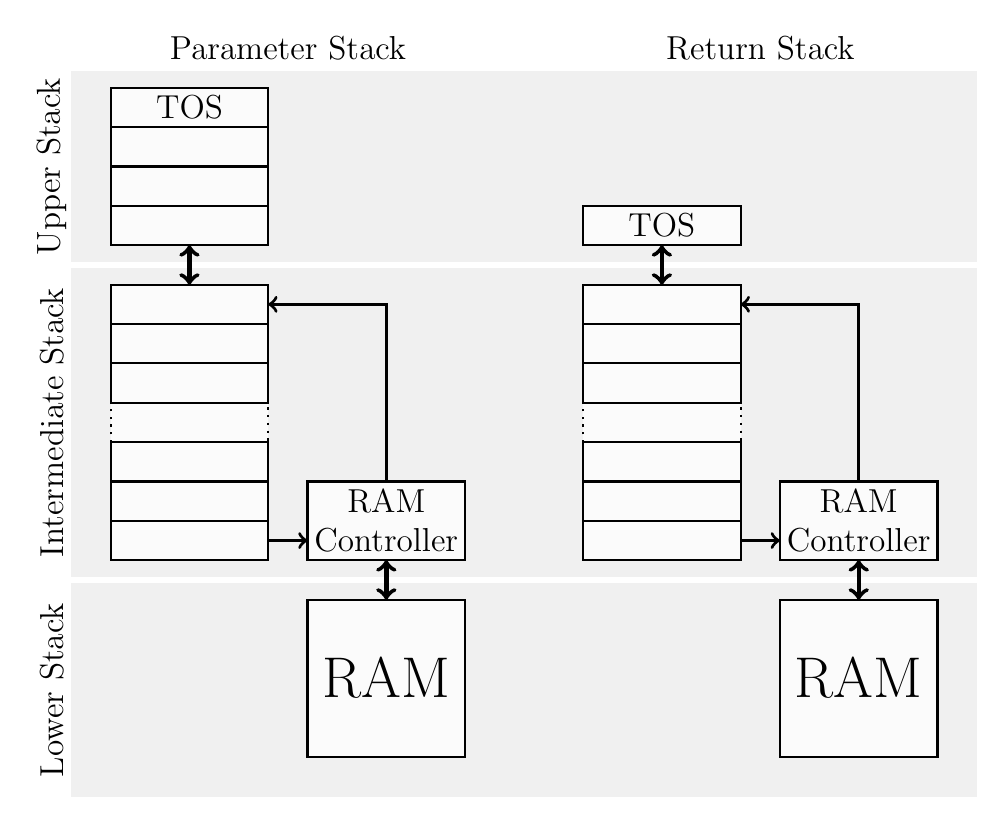
\begin{tikzpicture}

        %Common  stack structure
        \newsavebox{\comstastruc}
        \savebox{\comstastruc}{
          %RAM
          \draw [thick, fill=gray!3] (2.5,0) rectangle (4.5,2);
          \node at (3.5,1) {\huge{RAM}};
          %RAM controller
          \draw [thick, fill=gray!3] (2.5,2.5) rectangle (4.5,3.5);
          \node at (3.5,3)   {
            \begin{minipage}[c]{10em}
              \begin{center}
                \large{RAM}\\
                \large{Controller}
              \end{center}
          \end{minipage}};
          \draw [ultra thick, <->] (3.5,2.5) --  (3.5,2);
          %Intermediate stack
          \draw [thick, fill=gray!3, dotted](0,4)   rectangle (2,4.5);
          \draw [thick, fill=gray!3]        (0,2.5) rectangle (2,3);
          \draw [thick, fill=gray!3]        (0,3)   rectangle (2,3.5);
          \draw [thick, fill=gray!3]        (0,3.5) rectangle (2,4);
          \draw [thick, fill=gray!3]        (0,4.5) rectangle (2,5);
          \draw [thick, fill=gray!3]        (0,5)   rectangle (2,5.5);
          \draw [thick, fill=gray!3]        (0,5.5) rectangle (2,6);          
          \draw [very thick, ->]            (2,2.75) --  (2.5,2.75);
          \draw [very thick, <-]            (2,5.75) --  (3.5,5.75) -- (3.5,3.5);
          %Upper stack
          \draw [thick, fill=gray!3]        (0,6.5) rectangle (2,7);
          \draw [ultra thick, <->] (1,6.5) -- (1,6);
        }
        %Lower stack
        \draw [gray!12, fill=gray!12](0.5,0)   rectangle (12,2.7);
        \node [rotate=90] at (0.25,1.35) {\large{Lower Stack}};

        %Intermediate stack
        \draw [gray!12, fill=gray!12](0.5,2.8) rectangle (12,6.7);
        \node [rotate=90] at (0.25,4.75) {\large{Intermediate Stack}};

        %Upper stack
        \draw [gray!12, fill=gray!12](0.5,6.8) rectangle (12,9.2);
        \node [rotate=90] at (0.25,8) {\large{Upper Stack}};

        %Parameter stack
        \node at (1,0.5) {\usebox{\comstastruc}};
        \draw [thick, fill=gray!3]        (1,7.5) rectangle (3,8);
        \draw [thick, fill=gray!3]        (1,8)   rectangle (3,8.5);
        \draw [thick, fill=gray!3]        (1,8.5) rectangle (3,9);
        \node at (2,8.75) {\large{TOS}};
        \node at (3.25,9.5) {\large{Parameter Stack}};
                
        %Parameter stack
        \node at (7,0.5) {\usebox{\comstastruc}};
        \node at (8,7.25) {\large{TOS}};
        \node at (9.25,9.5) {\large{Return Stack}};

        
       \end{tikzpicture}
    }
  }
  \caption{Stack Architecture}
  \label{stacks:fig}
  \end{center}
\end{figure}

\subsection{Parameter Stack}
\label{stacks:ps}

The \gls{us} of the \gls{ps} contains is four \glspl{cell} deep and contains the
most recent data entries. It's purpose is to perform stack and ALU operations
(see \secref{opcodes:stack} and \secref{opcodes:alu}).
When the capacity of the \gls{us} is exceeded, older data entries are transferred
to the \gls{is}.

The \gls{is} serves as a buffer between the \gls{us} and the \gls{ls} which resides
in \gls{ram}. The purpose of the \gls{is} is to minimize \gls{ram} traffic to and
from the \gls{ls}.
Push operation to the \gls{is} are only propagated to the \gls{ls}, when the buffer
capacity is exceeded. Pull operations are onle propagated, when the \gls{is} is empty.
\Gls{stack} fluctuations within the buffer capacity are not visible to the \gls{ls}.

The \gls{ls} is a region of the \gls{ram}, which is managed by the memory controller
of the \gls{is}.

\subsection{Return Stack Stack}
\label{stacks:ps}

The \gls{us} of the \gls{ps} has the capacity of one \gls{cell}. The \gls{is} and
\gls{ls} are similar to the ones of the \gls{ps}.
